\section{误差来自何处}

简单的模型有着较大的偏差(bias),使用相同模型,不同数据得到的最优函数$f^*$的取值区间可能不包括理论最优解$\hat{f}$,因此偏差较大。而对于过于复杂的模型,又容易产生对数据的过拟合,出现大的方差。
对于复杂模型,多次实验求取的模型均值能够更加接近理论解$\hat{f}$,但同时一个模型对于新的测试集数据容易产生大的误差,此时误差主要来自方差(variance)。偏差与误差的形象解释如图\ref{fig:bias_and_variance}所示:
\begin{figure}
	\centering

	{\subcaptionbox{误差之偏差}{%
	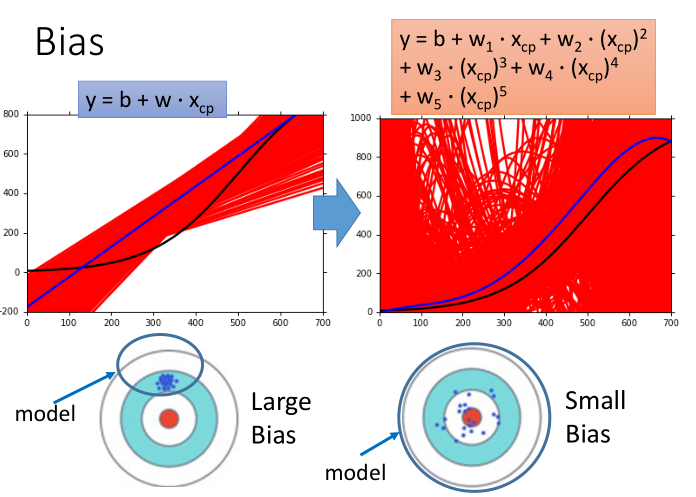
\includegraphics[scale=0.4]{pic/bias.png}}\qquad
	\subcaptionbox{误差之方差}{%
	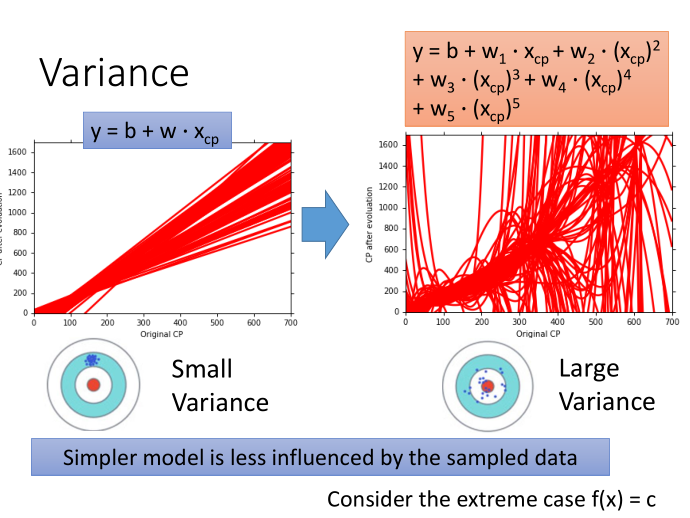
\includegraphics[scale=0.4]{pic/variance.png}}
	}
	\caption{bias VS variance}
	\label{fig:bias_and_variance}
\end{figure}

针对方差和偏差导致的过拟合和欠拟合问题,分别通过以下方法改善:
\begin{itemize}
\item 偏差
	\subitem 重新修正模型,使用更加复杂的模型
	\subitem 使用更多的样本特征
\item 方差
	\subitem 增加样本数据量
	\subitem 模型正则化
\end{itemize}

对于在实际训练模型过程中,训练集上得到的模型,通过 public 测试集得到的错误率与在 private 测试集上的错误率不一定是一致的。为了在没有 private 测试集的前提下能够较好的预知错误率,可以通过在训练集上划分训练集和验证集加以实现。
如图\subref{subfig:validation}所示:同时为了充分利用训练集数据可以采用 N-折交叉验证。模型的正确率由 N 个正确率的均值决定。如图\subref{subfig:N_fold_cross_validation}所示。
\begin{figure}
	\centering

	{\subcaptionbox{划分验证集\label{subfig:validation}}{%
	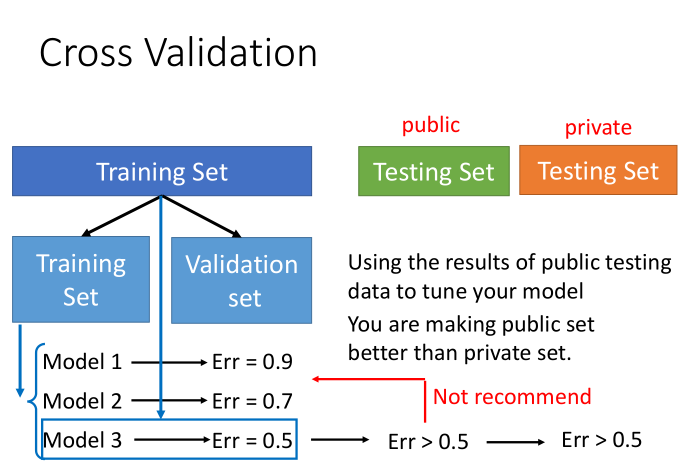
\includegraphics[scale=0.4]{pic/cross_validation.png}}\qquad
	\subcaptionbox{N-折交叉验证\label{subfig:N_fold_cross_validation}}{%
	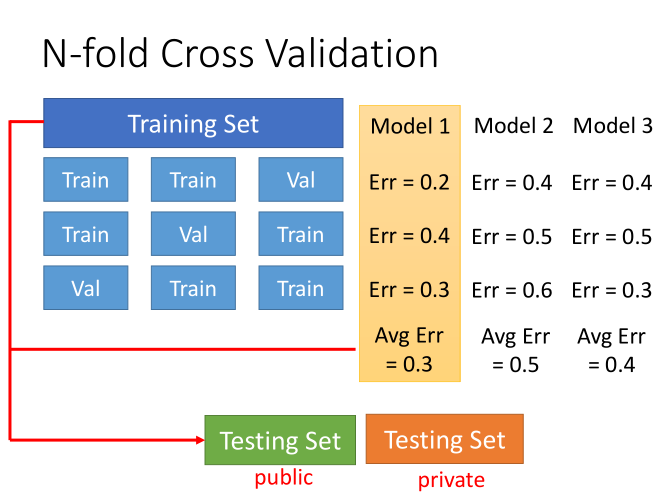
\includegraphics[scale=0.4]{pic/N_fold_cross_validation.png}}
	}
	\caption{交叉验证}
	\label{fig:cross_validation}
\end{figure}
